\documentclass{article}
\usepackage[latin1]{inputenc}
\usepackage{german}
\usepackage{fancyvrb}
\usepackage{amssymb}
\usepackage{a4wide}
\usepackage{epsfig}

\def\pair(#1,#2){\langle #1, #2 \rangle}
\newcommand{\qote}[1]{``\texttt{#1}''}

\newcounter{aufgabe}
\newcommand{\exercise}{\vspace*{0.3cm}
\stepcounter{aufgabe}

\noindent
\textbf{Aufgabe \arabic{aufgabe}}: }

\renewcommand{\labelenumi}{(\alph{enumi})}
\renewcommand{\labelenumii}{\arabic{enumii}.}

\begin{document}


\noindent
{\large L\"osungen zu den Aufgaben zur Vorlesung  ``{\sl Formale Sprachen}''}
\vspace{0.5cm}

\noindent
\exercise
Eine m\"ogliche L\"osung sehen Sie nachstehend:
\begin{Verbatim}[ frame         = lines, 
                  framesep      = 0.3cm, 
                  labelposition = bottomline,
                  numbers       = left,
                  numbersep     = -0.2cm,
                  xleftmargin   = 0.8cm,
                  xrightmargin  = 0.8cm,
                ]
    %%
    
    %class Kasse
    %standalone
    
    %unicode
    
    %{
        double mCount = 0;
    %}
    
    %eof{
        System.out.println("Total: " + mCount); 
    %eof}
    
    %%
    
    ([1-9][0-9]*|[0-9])\.[0-9][0-9]  { mCount += new Double(yytext()); }
    .|\n                             { /* skip */                      }
\end{Verbatim}

\exercise
\begin{enumerate}
\item Eine m\"ogliche L\"osung ist unten gezeigt. Beachten Sie, dass bei dieser L\"osung
      der Wert $\delta(q_2,a)$ undefiniert ist.

      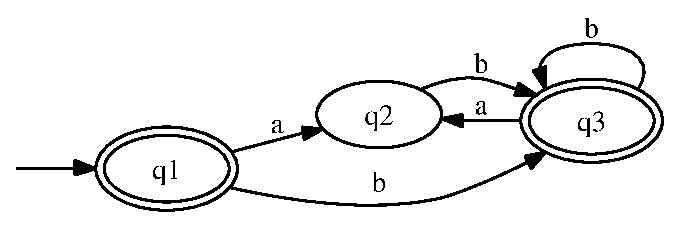
\epsfig{file=Abbildungen/graph-a.eps, scale=0.6}
 
      \textbf{Bemerkung}: Der Zustand $q_2$ ist der einzige Zustand, der nicht-akzeptierend ist. 
      Wir gelangen sowohl von $q_1$ als auch von $q_3$ in diesen Zustand,
      wenn wir ein ``\texttt{a}'' lesen.  Lesen wir anschlie{\ss}end ein ``\texttt{b}'',
      so gelangen wir wie vorgeschrieben in den akzeptierenden Zustand $q_3$ in dem wir
      dann noch beliebig viele ``\texttt{b}''s einlesen k\"onnen.   Falls wir im Zustand
      $q_2$ ein ``\texttt{a}'' lesen, so stirbt der Automat, aber das ist auch richtig so,
      denn auf jedes ``\texttt{a}'' soll ja ein ``\texttt{b}'' folgen.
\item Die Sprache wird von dem regul\"aren Ausdruck $(b+ab)^*$ beschrieben.
\item Die unten stehende Abbildung zeigt eine L\"osung.  Die unbeschrifteten Kanten sind
      $\varepsilon$-\"Uberg\"ange.

      \epsfig{file=Abbildungen/graph-c.eps, scale=0.6}
\item Wir definieren die Zust\"ande wir folgt:
      \begin{enumerate}
      \item $S_0 = \{ q_0, q_1, q_2, q_4, q_8 \}$,
      \item $S_1 = \Delta(S_0, a) = \{ q_5 \}$,
      \item $S_2 = \Delta(S_0, b) = \{ q_3, q_7, q_1, q_2, q_4, q_8 \}$,
      \item $S_3 = \Delta(S_1, a) = \{ \}$,
      \item $S_4 = \Delta(S_1, b) = \{ q_6, q_7, q_1, q_2, q_4, q_8 \}$,
      \item $\Delta(S_2, a) = \{ q_5 \} = S_1$,
      \item $\Delta(S_2, b) = \{ q_3, q_7, q_1, q_2, q_4, q_8 \} = S_2$,
      \item $\Delta(S_3, a) = \{ \}$,
      \item $\Delta(S_3, b) = \{ \}$,
      \item $\Delta(S_4, a) = \{ q_5 \} = S_1$,
      \item $\Delta(S_4, b) = \{ q_3, q_7, q_1, q_2, q_4, q_8 \} = S_2$.
      \end{enumerate}
      Der Startzustand ist $S_0$, die Zust\"ande $S_0$, $S_2$ und $S_4$ sind akzeptierend.
      Die folgende Abbildung zeigt den deterministischen Automaten.

      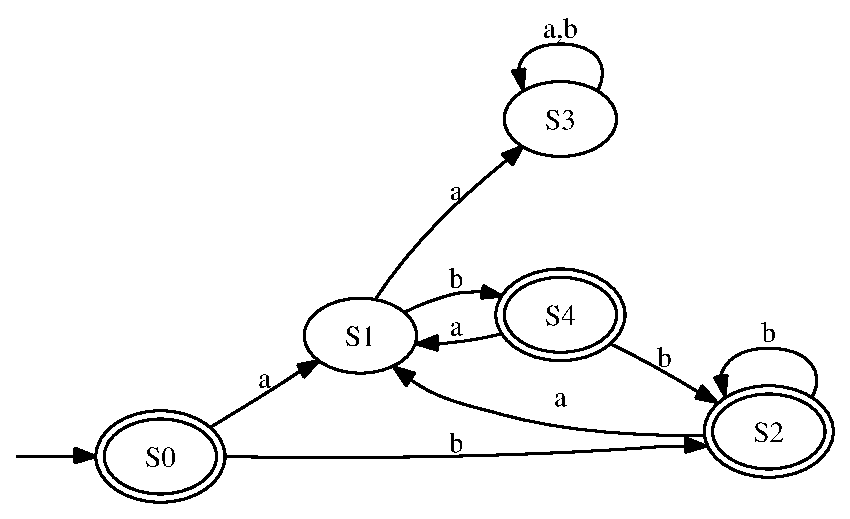
\epsfig{file=Abbildungen/graph-d.eps, scale=0.6}
\item Wir gehen wir im Skript beschrieben vor und erstellen eine Tabelle.
      \begin{enumerate}
      \item Im ersten Schritt erkennen wir, dass die akzeptierenden Zust\"ande $S_0$,
            $S_2$ und $S_4$ von den nicht-akzeptierenden Zust\"anden $S_1$ und $S_3$ unterscheidbar sind.
            Damit hat der erste Entwurf unserer  Tabelle die folgende Gestalt:
            \begin{center}        
            \begin{tabular}[t]{|l||l|l|l|l|l|}
            \hline
                  &$S_0$&$S_1$&$S_2$&$S_3$&$S_4$ \\
            \hline
            \hline
            $S_0$ &$\sim$&  1  &     &  1  &     \\
            \hline
            $S_1$ &  1  &$\sim$&  1  &     &  1  \\
            \hline
            $S_2$ &     &  1  &$\sim$&  1  &     \\
            \hline
            $S_3$ &  1  &     &  1  &$\sim$&  1  \\
            \hline
            $S_4$ &     &  1  &     &  1  &$\sim$\\
            \hline
            \end{tabular}
            \end{center}
      \item Als n\"achstes erkennen wir, dass die Zust\"ande $S_1$ und $S_3$ unterscheidbar sind,
            denn es gilt 
            \\[0.2cm]
            \hspace*{1.3cm}
            $\delta(S_1,b) = S_4$, \quad $\delta(S_3,b) = S_3$ \quad und \quad $S_4 \not\sim S_3$.
            \\[0.2cm]
            Auf der anderen Seite sehen wir, dass die Zust\"ande $S_0$ und $S_2$ nicht
            unterscheidbar sein k\"onnen, denn es gilt
            \\[0.2cm]
            \hspace*{1.3cm}
            $\delta(S_0,a) = S_1 = \delta(S_2,a)$ \quad und 
            $\delta(S_0,b) = S_2 = \delta(S_2,b)$.
            \\[0.2cm]
            Wir folgern $S_0 \sim S_2$.  Genauso sehen wir, dass $S_0 \sim S_4$ ist, denn
            es gilt
            \\[0.2cm]
            \hspace*{1.3cm}
            $\delta(S_0,a) = S_1 = \delta(S_4,a)$ \quad und 
            $\delta(S_0,b) = S_2 = \delta(S_4,b)$.
            \\[0.2cm]
            Aus $S_0 \sim S_2$ und $S_0 \sim S_4$ folgt sofort $S_2 \sim S_4$,
            Damit haben wir jetzt alle m\"oglichen \"Aquivalenzen untersucht und unsere
            Tabelle hat die folgende Form:
            \begin{center}        
            \begin{tabular}[t]{|l||l|l|l|l|l|}
            \hline
                  &$S_0$&$S_1$&$S_2$&$S_3$&$S_4$ \\
            \hline
            \hline
            $S_0$ &$\sim$&  1  &$\sim$&  1  &$\sim$ \\
            \hline
            $S_1$ &  1  &$\sim$&  1  &  2  &  1  \\
            \hline
            $S_2$ &$\sim$&  1  &$\sim$&  1  &$\sim$ \\
            \hline
            $S_3$ &  1  &  2  &  1  &$\sim$&  1  \\
            \hline
            $S_4$ &$\sim$&  1  &$\sim$&  1  &$\sim$\\            
            \hline
            \end{tabular}
            \end{center}
      \end{enumerate}
      Die Zust\"ande $S_0$, $S_2$ und $S_4$ sind also paarweise \"aquivalent.
      Die nachstehende Abbildung zeigt die L\"osung.  

      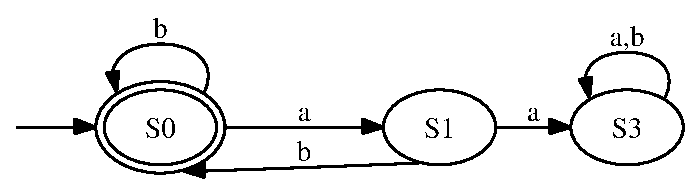
\epsfig{file=Abbildungen/graph-e.eps, scale=0.6}
\end{enumerate}

\exercise
Wir f\"uhren den Beweis indirekt und nehmen an, dass $L_P$ eine regul\"are Sprache w\"are.
Nach dem Pumping-Lemma gibt es dann eine nat\"urliche Zahl $n$, so dass gilt:
\\[0.2cm]
\hspace*{0.5cm}
  $\forall s \in L_P : \bigl(|s| \geq n \rightarrow \exists u,v,w\in \Sigma^* :
   s = uvw \wedge v \not= \varepsilon \wedge |uv| \leq n \wedge 
   (\forall h \in \mathbb{N}: uv^h w \in L_P)\bigr)
$.
\\[0.2cm]
In Worten hei{\ss}t dass: F\"ur alle $s \in L_P$, f\"ur die $|s| \geq n$ gilt, gibt es eine Zerlegung
\\[0.2cm]
\hspace*{1.3cm}
$s = uvw$,
\\[0.2cm]
so dass  $v \not= \varepsilon$ und $|uv| \leq n$ gilt.  Wir setzen nun
\\[0.2cm]
\hspace*{1.3cm}
$s := a^n b^{2 \cdot n} a^n$.
\\[0.2cm]
Dann gilt $s^r = s$ und damit $s \in L_P$.  Weiter ist $|s| = 4 \cdot n \geq n$.
Also gibt es nach dem Pumping-Lemma eine Zerlegung von $s$ der Form
\\[0.2cm]
\hspace*{1.3cm}
$a^nb^{2 \cdot n} a^n = uvw$
\\[0.2cm]
mit den Eigenschaften $v \not= \varepsilon$ und $|uv| \leq n$.  Aus $|uv| \leq n$ folgt, dass der
String $uv$ ganz in dem String $a^n$ enthalten ist.  Damit m\"ussen die Strings $u$, $v$ und $w$
folgende Form haben:
\\[0.2cm]
\hspace*{1.3cm}
$u = a^i$, \quad $v = a^j$ \quad und \quad $w = a^k b^{2 \cdot n} a^n$,
\\[0.2cm]
wobei dann
\\[0.2cm]
\hspace*{1.3cm}
$i + j + k = n$
\\[0.2cm]
gelten muss.  Wegen $v \not= \varepsilon$ wissen wir, dass $j > 0$ ist.
Wir betrachten jetzt den String $uw = u v^0 w$, der nach Aussage des Pumping-Lemmas in der Sprache
$L_P$ liegen muss.  Es gilt
\\[0.2cm]
\hspace*{1.3cm}
$uw = a^i a^k b^{2 \cdot n} a^n$.
\\[0.2cm]
Aus $i + j + k = n$ und $j > 0$ folgt offenbar
\\[0.2cm]
\hspace*{1.3cm}
$i + k \not= n$
\\[0.2cm]
und damit ist $uw$ keine Palindrom.
\pagebreak

\exercise
\begin{enumerate}
\item Wir setzen 
      $G = \langle \{ S, T \}, \{ \mathtt{a}, \mathtt{b}, \mathtt{c} \}, R, S \rangle$, 
      wobei die Regeln $R$ wie folgt 
      gegeben sind:
      \\[0.2cm]
      \hspace*{1.3cm} $S \rightarrow   \mathtt{a}S\mathtt{c} \mid T$, \\[0.2cm]
      \hspace*{1.3cm} $T \rightarrow \mathtt{b}T\mathtt{c} \mid \varepsilon$. 
      \\[0.2cm]
      Die m\"oglichen Ableitungen von $T$ haben die Form
      \\[0.2cm]
      \hspace*{1.3cm}
      $T \Rightarrow \mathtt{b}T\mathtt{c} \Rightarrow \mathtt{b}^2T\mathtt{c}^2
      \Rightarrow \cdots \Rightarrow \mathtt{b}^lT\mathtt{c}^l \Rightarrow \mathtt{b}^l\mathtt{c}^l$,
      \\[0.2cm]
      Dies zeigt, dass f\"ur die durch $T$ beschriebene Sprache folgendes gilt:
      \\[0.2cm]
      \hspace*{1.3cm}
      $L(T) = \{ \mathtt{b}^l \mathtt{c}^l \mid l \in \mathbb{N} \}$.
      \\[0.2cm]
      Die m\"oglichen Ableitungen von $S$ haben die Form
      \\[0.2cm]
      \hspace*{1.3cm}
      $S \Rightarrow \mathtt{a}S\mathtt{c} \Rightarrow \mathtt{a}^2S\mathtt{c}^2
      \Rightarrow \cdots 
      \Rightarrow \mathtt{a}^kS\mathtt{c}^k 
      \Rightarrow \mathtt{a}^kT\mathtt{c}^k 
      \Rightarrow^* 
      \mathtt{a}^k \mathtt{b}^l \mathtt{c}^l\mathtt{c}^k$.
      \\[0.2cm]
      Dies zeigt, dass f\"ur die durch $S$ beschriebene Sprache folgendes gilt:
      \\[0.2cm]
      \hspace*{1.3cm}
      $L(S) = \{ \mathtt{a}^k \mathtt{b}^l \mathtt{c}^{l+k}\mid l \in \mathbb{N} \}$.
\item Wir k\"onnen die Sprache $L_2$ auf die Sprache $L_1$ zur\"uck f\"uhren, denn wenn
      $h \geq k+ l$ ist, hei{\ss}t dies nichts anderes als dass es ein $j \in \mathbb{N}$
      gibt, so dass $h = k + l + j$ gilt.  Damit haben wir
      \\[0.2cm]
      \hspace*{1.3cm}
      $L_2 = \{ \mathtt{a}^k \mathtt{b}^l \mathtt{c}^{l+k}\mathtt{c}^j\mid l \in
      \mathbb{N} \wedge j \in \mathbb{N} \}$.
      \\[0.2cm]
      Dies zeigt, dass die W\"orter aus $L_2$ aus W\"ortern von $L_1$ bestehen, an die noch
      der Buchstabe ``\texttt{c}'' beliebig oft herangeh\"angt wird. Dies f\"uhrt zu folgender
      Grammatik:
      \\[0.2cm]
      \hspace*{1.3cm}
      $G = \langle \{ \widehat{S}, S, T, C \}, \{ \mathtt{a}, \mathtt{b}, \mathtt{c} \}, R, 
       \widehat{S} \rangle$, 
      \\[0.2cm]
      wobei die Regeln wie folgt gegeben sind:
      \\[0.2cm]
      \hspace*{1.3cm} $\widehat{S} \rightarrow SC$,                           \\[0.2cm]
      \hspace*{1.3cm} $S \rightarrow   \mathtt{a}S\mathtt{c} \mid T$,         \\[0.2cm]
      \hspace*{1.3cm} $T \rightarrow \mathtt{b}T\mathtt{c} \mid \varepsilon$,  \\[0.2cm]
      \hspace*{1.3cm} $C \rightarrow \mathtt{c}C \mid \varepsilon$. 
      \\[0.2cm]
\end{enumerate}
\pagebreak

\exercise
Im Skript hatten wir gesehen, dass  Regeln der Form 
\\[0.2cm]
\hspace*{1.3cm} 
$A \rightarrow A \beta_1 \mid \cdots \mid A \beta_k  \mid \gamma_1 \mid \cdots \mid \gamma_l$
\\[0.2cm]
durch Einf\"uhren einer neuen Variablen $L$ in die folgenden nicht-links-rekursiven Regeln
\"uberf\"uhrt werden k\"onnen:
\\[0.2cm]
\hspace*{1.3cm}
$
\begin{array}[t]{lcl}
A & \rightarrow & \gamma_1\;L \;\mid\; \gamma_2\;L \;\mid\; \cdots \;\mid\; \gamma_l\;L  \\[0.2cm]
L & \rightarrow & \beta_1 \;L \;\mid\; \beta_2 \;L \;\mid\; \cdots \;\mid\; \beta_k \;L \;\mid\; \varepsilon
\end{array}
$
\\[0.2cm]
Wir f\"uhren also drei neue syntaktische Variablen $L_S$, $L_A$ und $L_B$ ein
und erhalten dann die folgenden Regeln:
\\[0.2cm]
\hspace*{1.3cm}
$
\begin{array}[t]{lcl}
  S   & \rightarrow & a B S L_S \mid L_S          \\
  L_S & \rightarrow & a b L_S \mid \varepsilon \\[0.2cm]
  A   & \rightarrow & b L_A                    \\
  L_A & \rightarrow & a A L_A \mid \varepsilon \\[0.2cm] 
  B   & \rightarrow & a L_B                    \\
  L_B & \rightarrow & a B L_B \mid \varepsilon
\end{array}
$

\exercise
\begin{enumerate}
\item Die Grammatik $G = \langle \{E\}, \{N\}, R, E \rangle$ , bei der die Regeln $R$ wie folgt
      gegeben sind, leistet das Gew\"unschte:
      \\[0.2cm]
      \hspace*{1.3cm}
      \begin{array}[t]{lcl}
        E & \rightarrow & \texttt{'+'}\; E\; E  \\
          & \mid        & \texttt{'-'}\; E\; E  \\
          & \mid        & \texttt{'*'}\; E\; E  \\
          & \mid        & \texttt{'/'}\; E\; E  \\
          & \mid        & \texttt{N}
      \end{array}
      \\[0.2cm]
      

\item Ein \textsc{Antlr}-Programm k\"onnte wie folgt aussehen:
\begin{Verbatim}[ frame         = lines, 
                  framesep      = 0.3cm, 
                  labelposition = bottomline,
                  numbers       = left,
                  numbersep     = -0.2cm,
                  xleftmargin   = 0.0cm,
                  xrightmargin  = 0.0cm,
                ]
    grammar Program;
    
    program : expr { System.out.println($expr.result); } ;
    
    expr returns [int result]
         : '+' e1 = expr e2 = expr { $result = $e1.result + $e2.result; } 
         | '-' e1 = expr e2 = expr { $result = $e1.result - $e2.result; } 
         | '*' e1 = expr e2 = expr { $result = $e1.result * $e2.result; } 
         | '/' e1 = expr e2 = expr { $result = $e1.result / $e2.result; } 
         | NUMBER { $result = new Integer($NUMBER.text); }
         ;
    
    NUMBER: ('0'..'9')|('1'..'9')('0'..'9')*;
    WS    : (' '|'\t'|'\n'|'\r') { skip(); };
\end{Verbatim} 
\end{enumerate} %$
\pagebreak

\exercise
\begin{enumerate}
\item Es sei $\Sigma = \{a,b\}$. Wir definieren die Sprachen $L_1$ und $L_2$ wie folgt: 
      \\[0.2cm]
      \hspace*{1.3cm}
      $L_1 = \{ a^k b^l \mid k,l \in \mathbb{N} \}$ \quad und \quad
      $L_2 = \{ a^k b^l \mid k,l \in \mathbb{N} : k = l \}$.
      \\[0.2cm]
      Dann gilt offenbar 
      \\[0.2cm]
      \hspace*{1.3cm}
      $L_2 = L_1 \cap (\Sigma^* \backslash L)$.
      \\[0.2cm]
      Die Sprache $L_1$ ist offenbar regul\"ar, denn sie wird durch den regul\"aren Ausdruck
      $a^* b^*$ beschrieben.  Die Sprache $L_2$ ist identisch mit der Sprache
      \\[0.2cm]
      \hspace*{1.3cm}
      $\{ a^k b^k \mid k \in \mathbb{N} \}$ 
      \\[0.2cm]
      und von dieser Sprache haben wir bereits im Skript gezeigt, dass sie nicht regul\"ar ist.
      W\"are nun $L$ regul\"ar, so w\"are auch das Komplement von $L$, die Sprache
      $\Sigma^* \backslash L$ regul\"ar. Da der Schnitt zweier regul\"arer Sprache ebenfalls
      regul\"ar ist, w\"are dann auch $L_2$ regul\"ar, im Widerspruch zu dem in der Vorlesung gezeigten
      Ergebnis.
\item Wir geben eine Grammatik an, die diese Sprache erzeugt:
      \\[0.2cm]
      \hspace*{1.3cm}
      \begin{array}[t]{lcl}
        S & \rightarrow & A \mid B \\[0.2cm]
        A & \rightarrow & aG \mid aA \\[0.2cm]
        B & \rightarrow & Gb \mid Bb \\[0.2cm]
        G & \rightarrow & \varepsilon \mid aGb
      \end{array}
      \\[0.2cm]
      Die Idee hinter dieser Grammatik ist folgende:
      \begin{enumerate}
      \item $L(G) = \{ a^k b^l \mid k,l \in \mathbb{N} : k = l \}$, 
      \item $L(A) = \{ a^k b^l \mid k,l \in \mathbb{N} : k > l \}$,
      \item $L(B) = \{ a^k b^l \mid k,l \in \mathbb{N} : k < l \}$,
      \item $L(S) = \{ a^k b^l \mid k,l \in \mathbb{N} : k < l \vee k > l \}$.
      \end{enumerate}
\end{enumerate}
\pagebreak

\exercise
%\begin{enumerate}
Wir f\"uhren den Beweis indirekt und nehmen an, $L_{\mathbb{P}}$ w\"are regul\"ar.  Nach
dem Pumping-Lemma gibt es dann eine Zahl $n$, so dass es f\"ur alle Strings $s \in L_{\mathbb{P}}$, 
deren L\"ange gr\"o{\ss}er-gleich $n$ ist, eine Zerlegung
\\[0.2cm]
\hspace*{1.3cm}
$s = uvw$
\\[0.2cm]
mit den folgenden drei Eigenschaften gibt:
\begin{enumerate}
\item $v \not= \varepsilon$, 
\item $|uv| \leq n$ \quad und
\item $\forall h \in \mathbb{N}: u v^h w \in L_{\mathbb{P}}$.
\end{enumerate}
Wir w\"ahlen nun eine Primzahl $p$, die gr\"o{\ss}er-gleich  $n + 2$ ist und setzen $s = \mathtt{a}^p$.
Dann gilt $|s| = p \geq n$ und die Voraussetzung des Pumping-Lemmas ist erf\"ullt.
Wir finden also eine Zerlegung von $\mathtt{a}^p$ der Form
\\[0.2cm]
\hspace*{1.3cm}
$\mathtt{a}^p = uvw$ 
\\[0.2cm]
mit den oben angegebenen Eigenschaften.
Aufgrund der Gleichung $s = uvw$ k\"onnen die Teilstrings $u$, $v$ und $w$ nur aus dem
Buchstaben ``\texttt{a}'' bestehen.  Also gibt es nat\"urliche Zahlen $x$, $y$, und
$z$ so dass gilt:
\\[0.2cm]
\hspace*{1.3cm}
$u = \mathtt{a}^x$, \quad $v = \mathtt{a}^y$ \quad und \quad $w = \mathtt{a}^z$.
\\[0.2cm]
F\"ur  $x$, $y$ und $z$ gilt dann Folgendes:
\begin{enumerate}
\item $x + y + z = p$,
\item $y \not= 0$,
\item $x + y \leq n$,
\item $\forall h \in \mathbb{N}: x + h \cdot y + z \in \mathbb{P}$.
\end{enumerate}
Setzen wir in der letzten Gleichung f\"ur $h$ den Wert $(x + z)$ ein, so erhalten wir
\\[0.2cm]
\hspace*{1.3cm}
$x + (x + z)\cdot y + z \in P$.
\\[0.2cm]
Wegen $x + (x + z)\cdot y + z = (x + z) \cdot (1 + y)$ h\"atten wir dann
\\[0.2cm]
\hspace*{1.3cm}
$(x + z) \cdot (1 + y) \in \mathbb{P}$.
\\[0.2cm]
Das kann aber nicht sein, denn wegen $y > 0$ ist der Faktor $1 + y$ von 1
verschieden und wegen $x + y \leq n$ und $x + y + z = p$ und $p \geq n + 2$ wissen wir, dass
$z \geq 2$ ist, so dass auch der Faktor $(x + z)$ von 1 verschieden ist.  Damit kann das Produkt
$(x + z) \cdot (1 + y)$ aber keine Primzahl mehr sein und wir haben einen Widerspruch zu der
Annahme, dass $L_{\mathbb{P}}$ regul\"ar ist.
%\item Wir f\"uhren den Beweis indirekt und nehmen an, $L_{\mathbb{P}}$ w\"are kontextfrei.  Nach
%      dem Pumping-Lemma gibt es dann eine Zahl $n$, so dass es f\"ur alle Strings $s \in L_{\mathbb{P}}$, 
%      deren L\"ange gr\"o{\ss}er als $n$ ist, eine Zerlegung
%      \\[0.2cm]
%      \hspace*{1.3cm}
%      $s = uvwxy$
%      \\[0.2cm]
%      mit den folgenden drei Eigenschaften gibt:
%      \begin{enumerate}
%      \item $|vwx| \leq n$ \quad und
%      \item $vx \not= \varepsilon$, 
%      \item $\forall h \in \mathbb{N}: u v^h w x^h y \in L_{\mathbb{P}}$.
%      \end{enumerate}
%      Wir w\"ahlen nun eine Primzahl $p$, die gr\"o{\ss}er als $n+1$ ist und setzen $s = \mathtt{a}^p$.
%      Dann gilt $|s| = p > n$ und die Voraussetzung des Pumping-Lemmas ist erf\"ullt.
%      Wir finden also eine Zerlegung von $\mathtt{a}^p$ der Form
%      \\[0.2cm]
%      \hspace*{1.3cm}
%      $\mathtt{a}^p = uvwxy$ 
%      \\[0.2cm]
%      mit den oben angegebenen Eigenschaften.
%      Aufgrund der Gleichung $s = uvwxy$ k\"onnen die Teilstrings $u$, $v$, $w$, $x$ und $y$ nur aus dem
%      Buchstaben ``\texttt{a}'' bestehen.  Also gibt es nat\"urliche Zahlen $c$, $d$, $e$, $f$ und
%      $g$ so dass gilt:
%      \\[0.2cm]
%      \hspace*{1.3cm}
%      $u = \mathtt{a}^c$, \quad $v = \mathtt{a}^d$, \quad $w = \mathtt{a}^e$, \quad 
%      $x = \mathtt{a}^f$ \quad und \quad $y = \mathtt{a}^g$.
%      \\[0.2cm]
%      F\"ur die Zahlen $c$, $d$, $e$, $f$ und $g$ gilt dann Folgendes:
%      \begin{enumerate}
%      \item $c + d + e + f + g = p$,
%      \item $d + f \not= 0$,
%      \item $d + e + f \leq n$,
%      \item $\forall h \in \mathbb{N}: c + h \cdot d + e + h \cdot f + g \in \mathbb{P}$.
%      \end{enumerate}
%      Setzen wir in der letzten Gleichung f\"ur $h$ den Wert $(c + e + g)$ ein, so erhalten wir
%      \\[0.2cm]
%      \hspace*{1.3cm}
%      $c + (c + e + g) \cdot d + e + (c + e + g) \cdot f + g \in P$.
%      \\[0.2cm]
%      Wegen
%      \\[0.2cm]
%      \hspace*{1.3cm}
%      $c + (c + e + g) \cdot d + e + (c + e + g) \cdot f + g = (c + e + g) \cdot (1 + d + f)$ 
%      \\[0.2cm]
%      h\"atten wir dann
%      \\[0.2cm]
%      \hspace*{1.3cm}
%      $(c + e + g) \cdot (1 + d + f) \in \mathbb{P}$.
%      \\[0.2cm]
%      Das kann aber nicht sein, denn wegen $d + f > 0$ ist der Faktor $1 + d + f$ von 1
%      verschieden und wegen $d + e + f \leq n$ und $c + d + e + f + g = p$ und $p > n + 1$ wissen
%      wir, dass 
%      $c + g > 1$ ist, so dass auch der Faktor $(c + e + g)$ von 1 verschieden ist.  Damit kann das
%      Produkt $(c + e + g) \cdot (1 + d + f)$ aber keine Primzahl mehr sein und wir haben einen
%      Widerspruch zu der Annahme, dass $L_{\mathbb{P}}$ kontextfrei ist.
%\end{enumerate}

\exercise
Die Grammatik 
\\[0.2cm]
\hspace*{1.3cm}
 $G = \langle \{ E_1, E_2, \cdots, E_n \}, 
  \{ \textsc{Number}, \textsc{Var}, \mathtt{\#}_1, \cdots, \mathtt{\#}_n \}, R, E_1 \rangle$, 
\\[0.2cm]
deren Regeln wie folgt gegeben sind, leistet das Gew\"unschte:
\\[0.2cm]
\hspace*{1.3cm}
$
\begin{array}[t]{lcll}
E_k &\rightarrow& E_k \;\mathtt{\#}_k\; E_{k+1}  &  \\[0.2cm]
    &\mid       & E_{k+1}                    & \mbox{f\"ur alle $k \in \{1, \cdots, k-1\}$} \\[0.3cm]
E_n &\rightarrow& \textsc{Var}  \\
    &\mid       & \textsc{Number} 
\end{array}
$
\\[0.2cm]
Hier habe ich vorausgesetzt, dass die Operatoren $\texttt{\#}_k$ linksassoziativ sind.
\end{document}

%%% Local Variables: 
%%% mode: latex
%%% TeX-master: t
%%% End: 
